\documentclass[a4paper,10pt]{report}
\usepackage[cm]{fullpage}
\usepackage[utf8]{inputenc}
\usepackage{amsmath}
\usepackage{amsthm}
\usepackage{amssymb}
\usepackage{appendix}
\usepackage{booktabs}
\usepackage[table]{xcolor}
\usepackage{amssymb}
\usepackage{multirow}
\usepackage{fullpage}
\usepackage{float}
\usepackage{wrapfig}
\usepackage{subfig}
\usepackage{graphicx}
\usepackage{listings}
\usepackage{color}
\usepackage{textcomp}

\usepackage{sagetex}

\usepackage{hyperref}

\definecolor{listinggray}{gray}{0.9}
%\definecolor{lbcolor}{rgb}{0.9,0.9,0.9}

\addtolength{\voffset}{-10pt}

\hypersetup{colorlinks=false}
 
\lstset{
%	backgroundcolor=\color{lbcolor},
	tabsize=4,
%	rulecolor=,
	language=python,
        basicstyle=\scriptsize,
        upquote=true,
        aboveskip={1.5\baselineskip},
        columns=fixed,
        showstringspaces=false,
        extendedchars=true,
        breaklines=true,
        prebreak = \raisebox{0ex}[0ex][0ex]{\ensuremath{\hookleftarrow}},
%        frame=single,
        showtabs=false,
        showspaces=false,
        showstringspaces=false,
        identifierstyle=\ttfamily,
        keywordstyle=\color[rgb]{0,0,1},
        commentstyle=\color[rgb]{0.133,0.545,0.133},
        stringstyle=\color[rgb]{0.627,0.126,0.941},
} \hypersetup{colorlinks=false}

\renewcommand\chaptername{Esperimento}
 
\DeclareGraphicsExtensions{.pdf,.png,.jpg}


\author{Marco Giglio, Maria Cristina Fortuna, Riccardo Iaconelli}
% Title Page
\title{Relazioni dal Laboratorio di Fisica 2}

\begin{document}

\maketitle

\tableofcontents

% \chapter{Misura della velocità della luce}

L'obiettivo del nostro esperimento è misurare la velocità della luce $c$.

L'apparato di misurazione consiste principalmente in:
\begin{itemize}
 \item Un laser Elio-Neon ($\lambda=32$ nm).
 \item Uno specchio rotante a velocità angolare regolabile.
 \item Due lenti convergenti, di lunghezza focale $l_1 = 48mm$ e $l_2 = 252 mm$.
 \item Un microscopio con beam splitter e micrometro.
\end{itemize}

Lo specchio rotante viene fatto girare con velocità angolare $\omega_1$ in senso orario e $\omega_2$ in senso antiorario. Queste velocità angolari sono identiche nella maggior parte dei casi, e la loro differenza è trascurabile.

Chiamando $s_{cw}$ e $s_{ccw}$ rispettivamente le misure con specchio rotante in senso orario e antiorario, per come è orientata la strumentazione il numero
$$\Delta s = s_{cw} - s_{ccw}$$
deve essere positivo.

Purtroppo però non è questo il caso per qualche misura presa in mattinata, per ragioni sconosciute e che non siamo riusciti a riprodurre. Questi dati sono esclusi dalla misurazione in quanto evidenti errori, e sono mostrati in rosso nel grafico seguente
I dati sono molti, dunque forniamo qui soltanto una visione grafica, e lasciamo la tabella come allegato.

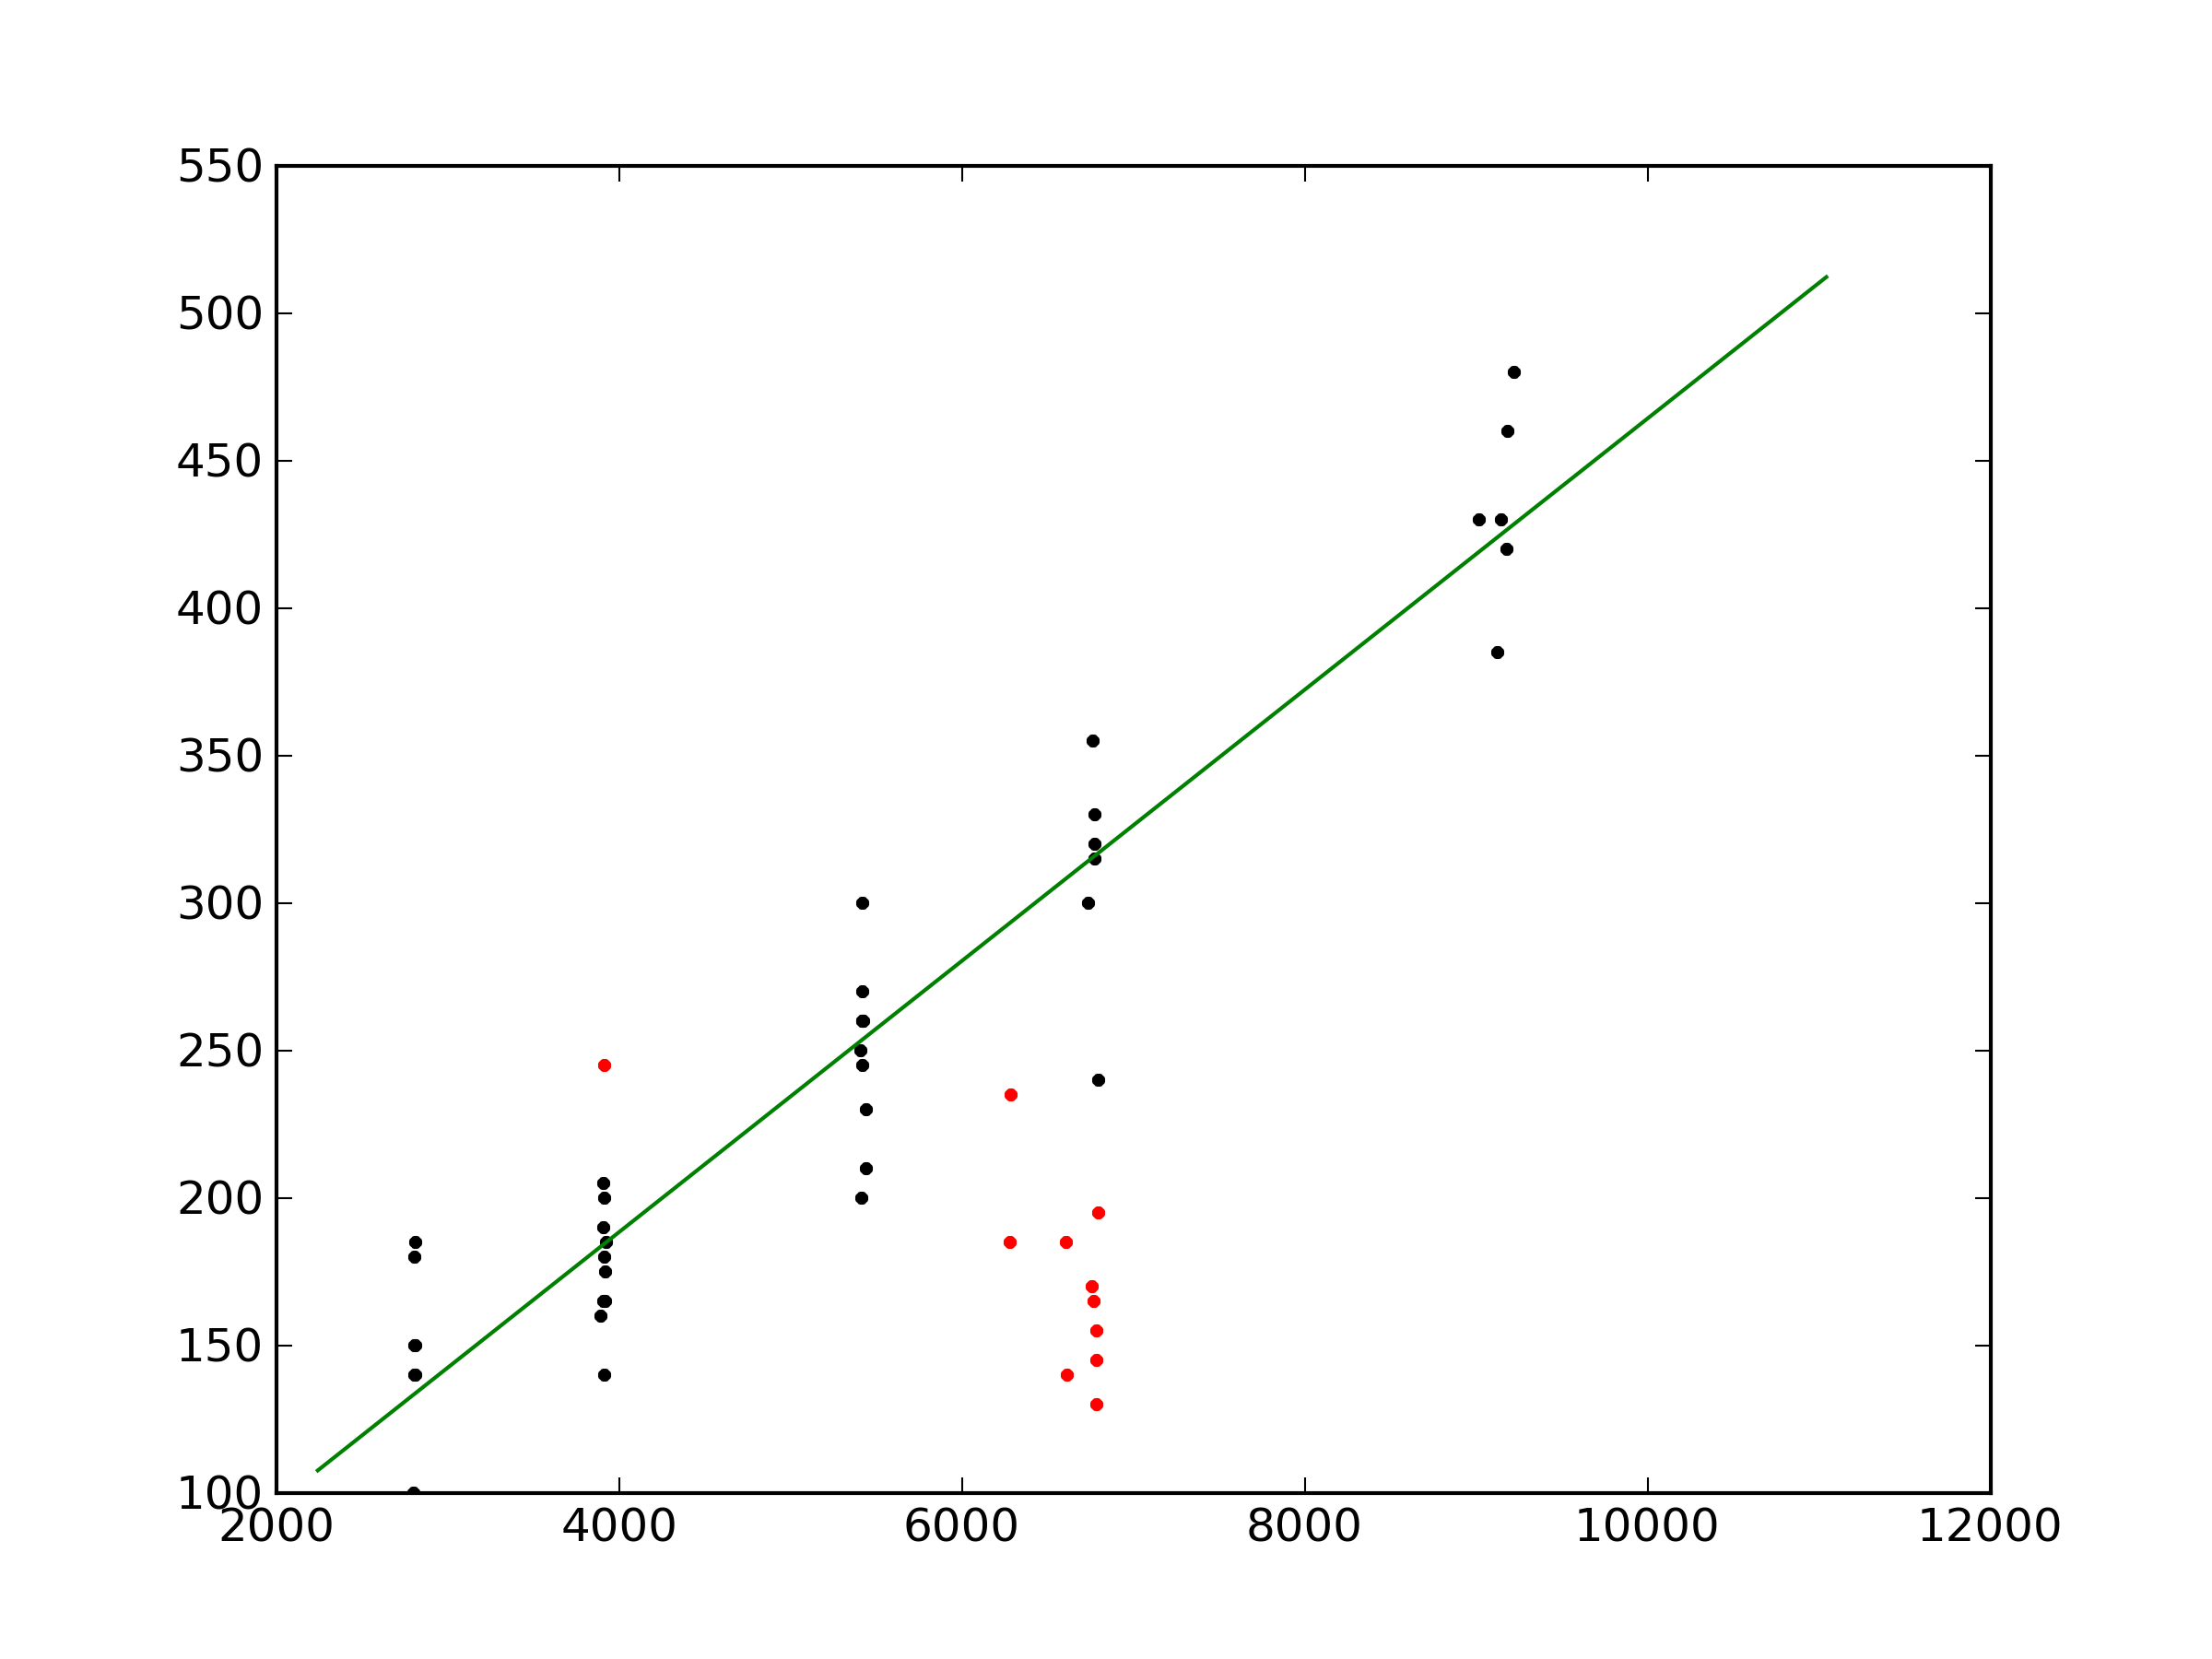
\includegraphics[scale=0.75]{grafici/C/dati.png}

\section{Analisi dati}

Chiamiamo $D = 13.480$m il cammino geometrico della luce per tornare allo specchio rotante, ovvero il doppio della distanza specchio rotante/specchio fisso; $A$ la distanza del punto di convergenza del fascio laser dalla lente $l_2$ e $B$ la distanza tra $l_2$ e lo specchio rotante. 

Per calcolare con precisione $A$, conoscendo la distanza focale di $l_2$, la ricaviamo dalla formula dei punti coniugati:
$$A=\frac{(B+D)f}{B+D-f} = 256\text{mm}$$


Per calcolare $c$, dobbiamo interpolare i dati presi nel modo seguente:
$$\Delta s = \frac{\tilde{A}}{c}\omega$$
ove
$$\tilde{A} = \frac{4*A*D^2}{2}$$

$\sage{2*e^2}$

La funzione che ci permetterà di calcolare $c$ è la seguente:

$$c = \frac{\tilde{A}}{m}$$
ove

Data una 
m=0.04594423946498933

Ricaviamo, tramite  il fit della funzione $V=R*I$" dove R è parametro da stimare, due resistenze ignote.


Misuro la resistenza interna del voltometro, mantenendo costante la ddp a $14.5\ V$ e variando la resistenza all'interno del circuito. 
Il voltmetro è in parallelo al circuito, perciò $R_i$:

$$R_i = \frac{RV}{RI-V} $$

dove R è la resistenza variabile, I la corrente nel circuito e $V= 14.5\ V$


La resistenza risulta $9.20 \pm 0.27 \ M \Omega$.


Misuriamo la resistenza interna dell'amperometro, che è collegato in serie al circuito. 

$$R_i = \frac{V-RI}{I}$$

In questo caso, R è fissato ($R=0.5 \Omega$) e sono V e I a variare

La resistenza interna risulta $11.42 \pm 0.45 \Omega$



Colleghiamo una piccola lampada a filamento al circuito, e verifichiamo che il suo comportamento resistivo non segue la legge di Ohm. 






\begin{sagesilent}
import matplotlib.pyplot as plt
import numpy as np
import scipy.optimize as opt
\end{sagesilent}


\chapter{Microonde}

\section{Riflessione}

Intendiamo verificare la legge di Cartesio utillizando una lastra di metallo come superficie rifelttente, posizionandola su un supporto magnetico sul goniometro.

\begin{equation}
sin(\theta_{incidente}) = sin(\theta_{rifratto})
\end{equation}

\begin{sagesilent}
dati = np.recfromcsv('dati/MICROONDE/cartesio.csv')
\end{sagesilent}

\begin{center}
\sagestr{stampa_dati(dati, r'$\theta_{inc}$ (rad) & $\theta_{rif}$ (rad) ' )}
\end{center}


\section{Misura della lunghezza d'onda}

\begin{sagesilent}
dati = np.recfromcsv('dati/MICROONDE/lambda.csv')

#Calcolo lambda:

d = np.array(dati['distanza'])
d.astype(float)
n = np.array(dati['enne'])
n.astype(float)
lam = 2*d/n
sigmad = 0.5
errlam = 2/n*sigmad

lmedia = np.average(lam)
confronto = abs(2.85-lmedia)

dati = ml.rec_append_fields(dati, 'lungonda', lam)

\end{sagesilent}

Se si pongono trasmettitore e ricevitore ad una distanza di $\frac{n \lambda}{2}$, si può osservare che essi generano onde stazionarie. Infatti le antenne delle due apparecchiature riflettono parzialmente le onde che ricevono, e se li si mette in una condizione tale per cui le onde riflesse hanno la stessa fase delle onde incidenti si osservano dei massimi, viceversa, se le fasi sono antagoniste, si avrà una condizione di nodo.
Ricaviamo la lunghezza d'onda posizionando emettitore e ricevitore ai capi del metro, e muovendo il ricevitore lungo questo osserviamo  il passaggio alterno per massimi e minimi di intensità. Ricaviamo $\lambda$ dalla nota formula per le onde stazionarie:
\begin{equation}
d = n\frac{\lambda}{2}
\label{d}
\end{equation}


\begin{center}
\sagestr{stampa_dati(dati, r'$d$ (cm) & $n$ (rad) & $\lambda$ (cm)' )}
\end{center}

Otteniamo una lambda media: $$ \sage{lmedia} \pm \sage{errlam}$$

%Dal confronto con la $\lambda$ (2.85 cm) teorica otteniamo: $\lambda_{teo} - \lambda_{cal} || = \sage{confronto} < 2 \sigma ( = 2 \sage{errlam} $


\section{Rifrazione attraverso un prisma}

In questa parte dell'esperienza si verifica la legge di snell:
\begin{equation}
\frac{sin(\theta_{i})}{sin(\theta_{r})} = \frac{n_2}{n_1}
\end{equation}
A tal fine posizioniamo una pedana di polistirolo sul goniometro, e vi poniamo sopra un prisma, sempre di polistirolo, contenente "styrene pellets". Si verifica la legge per vari massimi di intensità (Nota: $n_1$ = 1).

%Dati???

\section{Polarizzazione}

\begin{sagesilent}
#Calcolo dell'intensità con la legge di Malus

dati = np.recfromcsv('dati/MICROONDE/malus.csv')

izero = 8.75
gamma=dati['gamma']*3.14/180
iteorico = izero*(cos(gamma))**2

dati = ml.rec_append_fields(dati, 'iteo', iteorico)

\end{sagesilent}


Le microonde uscenti dal trasmettitore sono polarizzate linearmente, per cui soddisfano alla legge di Malus che lega l'intensità all'angolo tra la normale al ricevitore e la direzione dell'onda. Fissata una distanza, posizioniamo emettitore e ricevitore uno difronte all'altro e misuriamo la diminuzione d'intensità relativa al variare dell'angolo rispetto all'orizzontale di emettitore-ricevitore. Di seguito i dati letti sul multimetro a confronto con l'intensità teorica data dalla legge di Malus:

\begin{equation}
I = I_{0} cos^2 \gamma
\end{equation}

\begin{center}
%\sagestr{stampa_dati(dati, r'$I$ (Volt) & $\gamma$ (rad) & $I_{teorico}$ (Volt) ' )}
\end{center}


\section{Interferenza da doppia fenditura}
\begin{sagesilent}
dfen = np.recfromcsv("dati/microonde-doppiafen.csv")
dfen.sort()
var('x,a,w,t')
model(x, a, w, t) = a*sin(w*x+t)

def ff(x, a,w,t):
  f = fast_callable(model)
  return f(x,a,w,t)

#print dfen['angolo']
pars, pcov = opt.curve_fit(ff, np.array(dfen['angolo']), np.array(dfen['volt']), p0=[500., 50., 1.])

print pcov

print pars
plt.clf()
xin = np.arange(min(dfen['angolo']), 220, 1)
print "now"
yin = ff(xin, pars[0], pars[1], pars[2])
plt.plot(xin, yin)
plt.plot(dfen['angolo'], dfen['volt'], 'o--')

plt.savefig("grafici/microonde-doppiafend.png")
\end{sagesilent}


Utilizzando un supporto magnetico sul goniometro, montiamo tre lastre di metallo in modo da avere due
fenditure di circa 1,5 cm. Spostando il ricevitore si troviamo i massimi e i minimi di interferenza al fine di verificare la
loro posizione rispetto alla previsione teorica: $d \sin(\theta) = n \lambda$ (per i massimi, con d distanza delle fenditure, $\theta$ angolo
rispetto alla perpendicolare, n numero intero).

\includegraphics[scale=0.75]{grafici/microonde-doppiafend.png}

\section{Specchio di Lloyd}

\begin{sagesilent}
#Calcolo della lunghezza d'onda

dati = np.recfromcsv('dati/MICROONDE/lloyd.csv')

d = dati['delta']
enne = dati['n']

lam = 2*d/enne


dati = ml.rec_append_fields(dati, 'lung_onda', lam)

\end{sagesilent}

Posizioniamo emettitore e ricevitore a distanza di un circa un metro, uno dinnanzi all'altro. Su un secondo metro, perpendicolare alla direzione emettitore-ricevitore e passante per il goniometro, montiamo una lastra di metallo che funge da specchio: in tal modo generiamo un'interferenza dovuta alla differenza di cammino delle onde (una parte arriva direttamente al ricevitore, mentre altre onde percorrono il cammino dall'emettitore allo specchio e dallo specchio al ricevitore). Cerchiamo il minimo di intensità con lo specchio a distanza minima dal goniometro e raccogliamo i massimi di intensità al variare della distanza, per determinare $\lambda$ come in \ref{d}

\begin{center}
%\sagestr{stampa_dati(dati, r'$d$ (cm) & $n$ & $\lambda$ ' )}
\end{center}

\section{Diffrazione di Bragg}

\begin{sagesilent}
#Grafico dell'intensità in funzione dei gradi

dati = np.recfromcsv('dati/MICROONDE/bragg.csv')
plt.clf()
plt.plot(dati['theta'], dati['volt'],'ro')

plt.savefig("grafici/microonde-bragg.png")

\end{sagesilent}


Nell'ultima parte dell'esperimento ci proponiamo di verificare la legge di Bragg, 
\begin{equation}
n \lambda = 2 d \sin(\theta)
\end{equation}
la quale esprime analiticamente i fenomeni di interferenza causati dalla riflessione di onde su piani paralleli di un reticolo cristallino. Per riprodurre il fenomeno, facciamo incidere le microonde su un cubo di polistirolo su cui sono inserite su spaziature regolari delle sferette di acciaio.

Nella formula:\\
$\theta$ è l'angolo che il fascio incidente forma col piano cristallino\\
$\lambda$ è la lunghezza d'onda della radiazione\\
$d$ è la distanza tra due piani adiacenti\\
$n$ indica l'ordine della diffrazione (tipicamente solo quello per n=1 è apprezzabile).\\

La formula si spiega in maniera analitica considerando una differenza di cammino ottico pari a $2d\sin(\theta)$.


\includegraphics[scale=0.75]{grafici/microonde-bragg.png}

\section{Analisi dati}

\section{Allegato: dati}
\begin{sagesilent}
def stampa_dati(wa, header):
  s = r"\begin{tabular}{c*{" + "%d" % (len(wa.dtype)-1)
  s += r"}{|c}}"
  s += "%s \\\\" % (header)
  s += r"\midrule"
  for i in range(0, len(wa)):
    a = ["%s" %x for x in d[i]]
    s += "%s \\\\" % join(a, "&")
  s += r"\end{tabular}"
  return s
\end{sagesilent}

\begin{center}

% \sagestr{stampa_dati(d, r"Frequenza (Hz) & I (mA) & Valore mu & $V_{rms}$ (V)")}
\end{center}


%\chapter{Misura di resistenze}

L'obiettivo del nostro esperimento è misurare la validità della legge di Ohm per varie configurazioni di un circuito. 

Al fine di misurare corrente e potenziale, colleghiamo al nostro circuito due multimetri digitali. Il primo, che ha la funzione di voltmetro, lo poniamo ai capi della nostra resistenza collegato in parallelo; il secondo, in modalità amperometro, è posto in serie subito dopo la resistenza. 

Di seguito, gli strumenti con la loro precisione:
- Voltmetro (multimetro portatile), resistenza interna: 6 $M\Omega$
- Amperometro (multimetro da banco)
- Generatore da banco, resistenza interna ignota.


\section{Analisi dati}

Ricaviamo, tramite  il fit della funzione $V=R*I$" dove R è parametro da stimare, due resistenze ignote.

\subsection{Dati}

\begin{center}
\begin{tabular}{*{4}{c}}
Corrente1 & Potenziale1 & Corrente2 & Potenziale2\\
\midrule
396 & 201 & 3043 & 207\\
512 & 261 & 3667 & 250\\
706 & 360 & 4703 & 319\\
890 & 454 & 6365 & 432\\
1126 & 574 & 8984 & 609\\
1242 & 633 & 12326 & 836\\
1557 & 794 & 16898 & 1145\\
1812 & 925 & 340 & 24\\
1971 & 1005 & 725 & 50\\
2290 & 1168 & 966 & 66\\
2524 & 1286 & 1595 & 108\\
2850 & 1454 & 1822 & 124\\
3116 & 1589 & 2160 & 146\\
3407 & 1737 & 2302 & 157\\
3883 & 1980 & 2584 & 176\\
4229 & 2157 & 3100 & 211\\
4598 & 2344 & 3370 & 229\\
5072 & 2586 & 4036 & 274\\
5505 & 2807 & 4348 & 295\\
5820 & 2967 & 4596 & 312\\
6257 & 3191 & 4894 & 332\\
6738 & 3436 & 5578 & 379\\
7521 & 3835 & 6613 & 449\\
7880 & 4018 & 6963 & 473\\
8493 & 4331 & 7371 & 500\\
8852 & 4514 & 7864 & 533\\
9135 & 4658 & 8603 & 584\\
9431 & 4809 & 9066 & 615\\
9720 & 4957 & 9667 & 656\\
9972 & 5085 & 10816 & 733\\

\end{tabular}
\end{center}


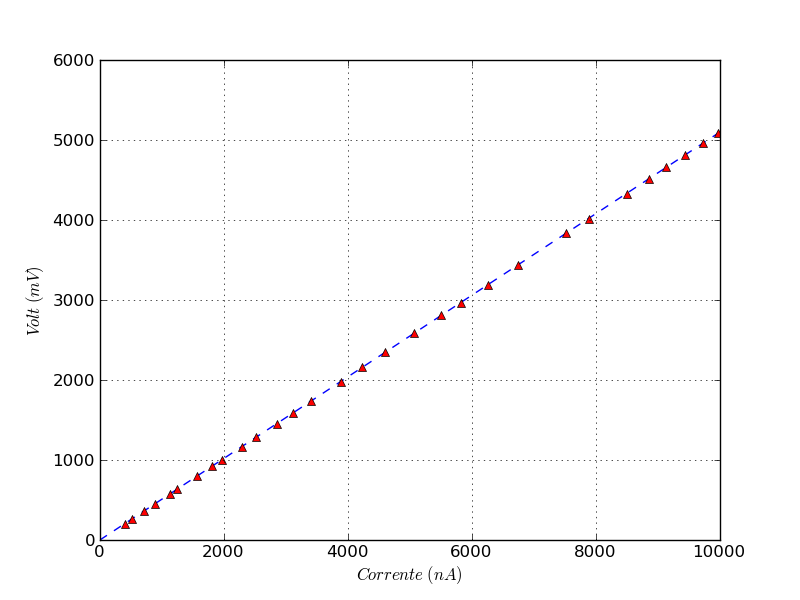
\includegraphics[scale=0.75]{grafici/C1/res1.png}
\
$\chi^2 = 5.76 $

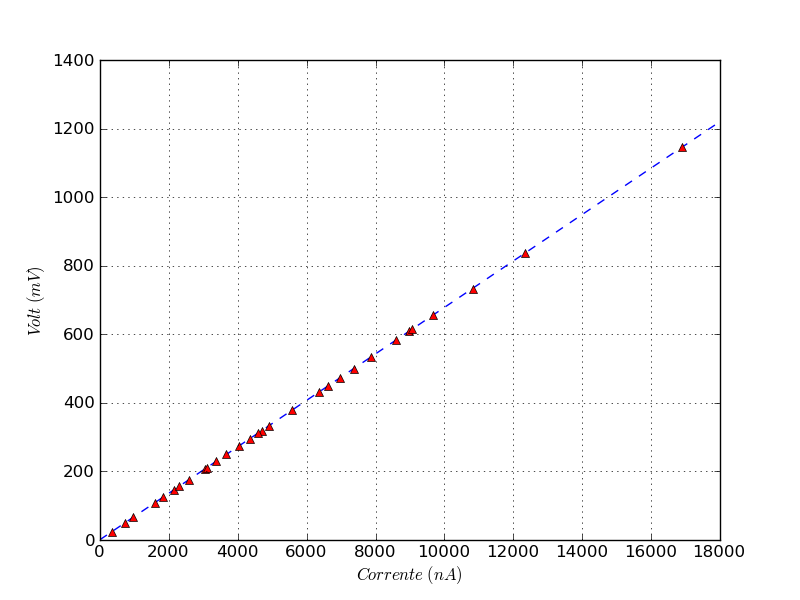
\includegraphics[scale=0.75]{grafici/C1/res2.png}

$\chi^2 = 4.88 $

Misuro la resistenza interna del voltometro, mantenendo costante la ddp a $14.5\ V$ e variando la resistenza all'interno del circuito. 
Il voltmetro è in parallelo al circuito, perciò $R_i$:

$$R_i = \frac{RV}{RI-V} $$

dove R è la resistenza variabile, I la corrente nel circuito e $V= 14.5\ V$

\begin{center}
\begin{tabular}{*{2}{c}}
Resistenza $M\Omega$ & Corrente $nA$\\
\midrule
7&      36\\
9&      32\\
10& 30\\
11&     29\\
12&     28\\
13&     27\\
14&     26\\
15&     26\\
16&     25\\
17&     24\\

\end{tabular}

La resistenza risulta $9.20 \pm 0.27 \ M \Omega$.


Misuriamo la resistenza interna dell'amperometro, che è collegato in serie al circuito. 

$$R_i = \frac{V-RI}{I}$$

In questo caso, R è fissato ($R=0.5 \Omega$) e sono V e I a variare
\begin{tabular}{*{2}{c}}
Volt $mV$ & Corrente $nA$\\
\midrule
22&      1769\\
40&      3271\\
60&      5047\\
105&     8938\\
133&     11201\\
142&     12021\\
164&     13882\\
174&     14745\\
208&     17604\\
232&     19671\\



\end{tabular}

La resistenza interna risulta $11.42 \pm 0.45 \Omega$


\end{center}


Colleghiamo una piccola lampada a filamento al circuito, e verifichiamo che il suo comportamento resistivo non segue la legge di Ohm. 

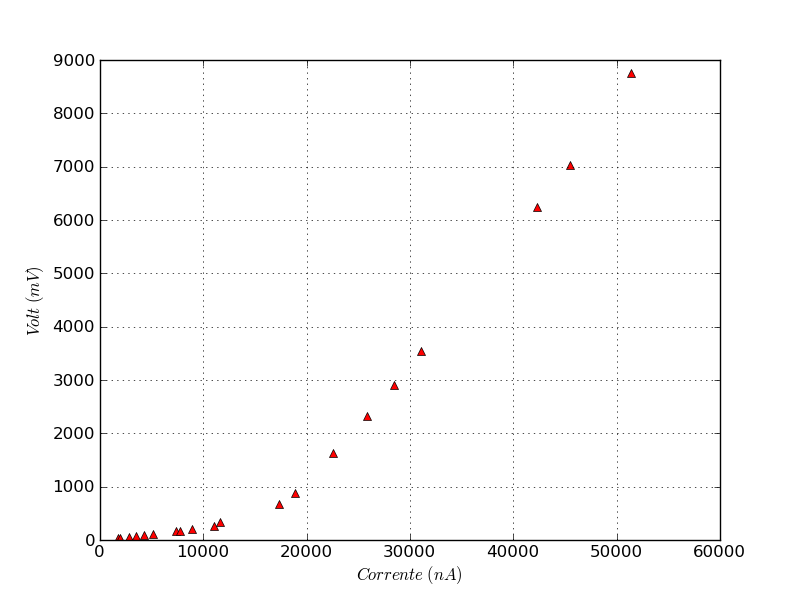
\includegraphics[scale=0.75]{grafici/C1/lampa.png}

La lampadina ha un comportamento non-ohmico nel momento in cui il filamento si scalda sufficientemente e inizia ad emettere luce ($500mV$).


\section{Partitore resistivo}

\subsection{Situazione senza carico}
\begin{center}
\begin{tabular}{*{2}{c}}
$V_{in}$ & $\frac{V_{in}}{V_{out}}$\\
\midrule
329.0 & 0.5015 \\
493.0 & 0.501 \\
544.0 & 0.5018 \\
618.0 & 0.5016 \\
667.0 & 0.5007 \\
776.0 & 0.5 \\
803.0 & 0.5006 \\
927.0 & 0.5005 \\
1078.0 & 0.5 \\
1285.0 & 0.4996 \\
\end{tabular}

\end{center}

$\chi^2=0.0169147373983$


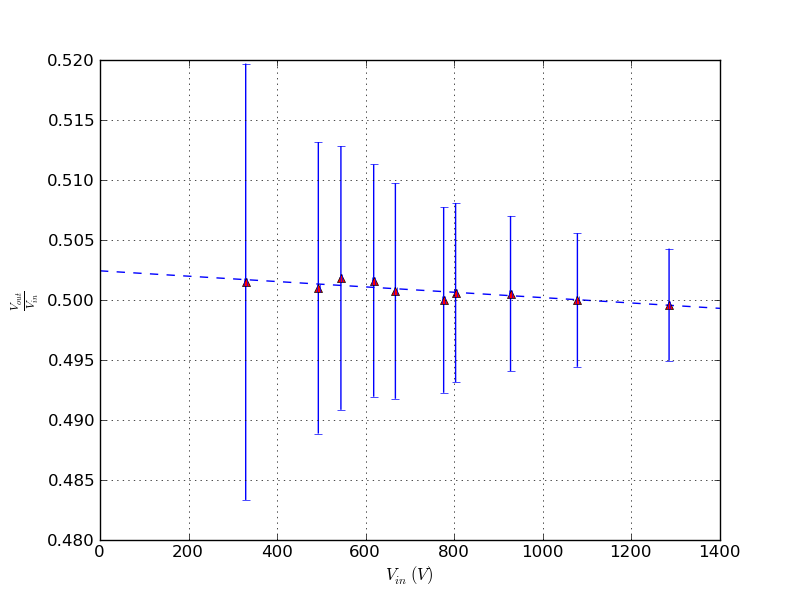
\includegraphics[scale=0.75]{grafici/C1/part1.png}

\subsection{Situazione con carico}
\begin{center}

\begin{tabular}{*{2}{c}}
$V_{in}$ & $\frac{V_{in}}{V_{out}}$\\
\midrule
220.0 & 3.1 \\
276.0 & 3.1051 \\
302.0 & 3.1126 \\
410.0 & 3.1073 \\
511.0 & 3.1115 \\
559.0 & 3.1055 \\
624.0 & 3.109 \\
752.0 & 3.109 \\
906.0 & 3.1093 \\
1036.0 & 3.111 \\
\end{tabular}

\end{center}
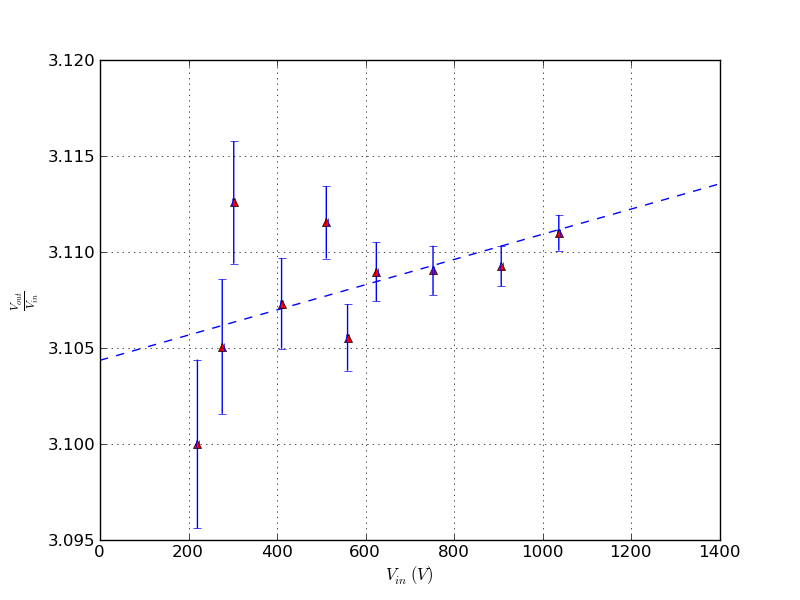
\includegraphics[scale=0.75]{grafici/C1/part2.png}

$\chi^2 = 12.9963702671$


\end{document} 



